\subsection{Voltage Balancing Scenario} \label{sec:sim_voltage_balance}

We now present the results of our second experiment, in which we incorporated two realizations of the \textit{LinDist3Flow} equations into OPFs that used DER resources to regulate and balance voltage magnitudes on an unbalanced radial distribution feeder.  Voltage balancing is an important objective as many three phase loads (induction motors for instance) are sensitive to high levels of imbalance.  Furthermore, many 3-phase voltage regulation equipment actuates based solely on single phase measurements.  Therefore, significant levels of imbalance can lead to improper operation of these devices. 

% \setlength{\abovedisplayskip}{2pt}
% \setlength{\belowdisplayskip}{2pt}
The results in this section expand on our previous work in \cite{arnold2015optimal} via adopting the iterative approach outlined in Section \ref{subsec:analysis_iter}. This simulation incorporated both constant power and constant impedance loads as defined in \cite{IEEEtestfeeder} for the 13 node case.  We define the problem as:
\begin{align}
% \begin{aligned}
  & \underset{u_{n}^{\phi},v_{n}^{\phi},y_{n}^{\phi},P_{n}^{\phi},Q_{n}^{\phi}} {\text{minimize}}
  % & & P_{0}\\
%   & & \sum_{n \in H} \left[ \sum_{ \substack{ {\phi, \psi} \\ {\phi \neq \psi} }} ( y_{n}^{\phi} - y_{n}^{\psi} )^{2} + \rho \sum_{\phi} \left| w_{n}^{\phi} \right|^{2} \right]  \\
  & & \sum_{n \in H} \left[ \sum_{\phi \neq \psi} ( y_{n}^{\phi} - y_{n}^{\psi} )^{2} + \rho \sum_{\phi} \left| w_{n}^{\phi} \right|^{2} \right] \nonumber \\
  & \text{subject to}
  & & ~\eqref{eq:mag_17}-\eqref{eq:pow_13}, \quad \underline{y} \le y_{n}^{\phi} \le \overline{y}, \nonumber \\
  & & & \left| w_{n}^{\phi} \right| \le \overline{w}, \quad \forall n \in H 
% \end{aligned}
\label{eq:OPF2}
\end{align}

\noindent where $\phi,\psi \in \{ a,b,c\}$. The parameter $\rho$ was chosen as $0.01$ and is a penalty on control action. We compared three cases to investigate the benefit of the iterative algorithm of Section \ref{subsec:analysis_iter}, as listed below:
\begin{itemize}
	\item[-] Case 0 - The uncontrolled, or base case (see Fig. \ref{fig:s2bc}).
	\item[-] Case 1 - OPF initialized as per assumptions outlined in Section \ref{subsec:analysis_nominal} with $\gamma_{n}^{\phi \psi} = \sigma \text{ or } \sigma^{2}$, and $\mathbb{L}_{mn} = \mathbb{H}_{mn}  = 0_{3 \times 1}$. See Fig. \ref{fig:s2c1}
    \item[-] Case 2 - OPF solved as outlined in Section \ref{subsec:analysis_iter}.  See Fig. \ref{fig:s2c3}
\end{itemize}

% \setlength{\abovedisplayskip}{0pt}
% \setlength{\belowdisplayskip}{0pt}

It should be noted that comparison of either case to an SDP formulation of \eqref{eq:OPF2} was not possible as it is not, to the authors knowledge, possible to formulate a semidefinite program with this objective function.

It can clearly be seen that for both Case 1 and Case 2, the voltage imbalance is drastically reduced compared to Case 0. In Case 1, the gap between phases a and b is reduced, however the magnitude of phase c remains lower throughout the feeder. In Case 2, the three phases are much more closely matched. We define voltage imbalance for the network as:
\begin{equation}
	J (\mathbb{Y}) = 
% 	\sum_{n \in H} \sum_{ \substack{ {\phi, \psi} \\ {\phi \neq \psi} }} ( y_{n}^{\phi} - y_{n}^{\psi} )^{2}
    \sum_{n \in H} \sum_{\phi \neq \psi} ( y_{n}^{\phi} - y_{n}^{\psi} )^{2}
    \label{eq:JV}
\end{equation}

% \setlength{\abovedisplayskip}{5pt}
% \setlength{\belowdisplayskip}{-50pt}
\setlength{\belowcaptionskip}{0pt}
\setlength{\textfloatsep}{5pt}
\begin{figure}[ht!]
	\centering
	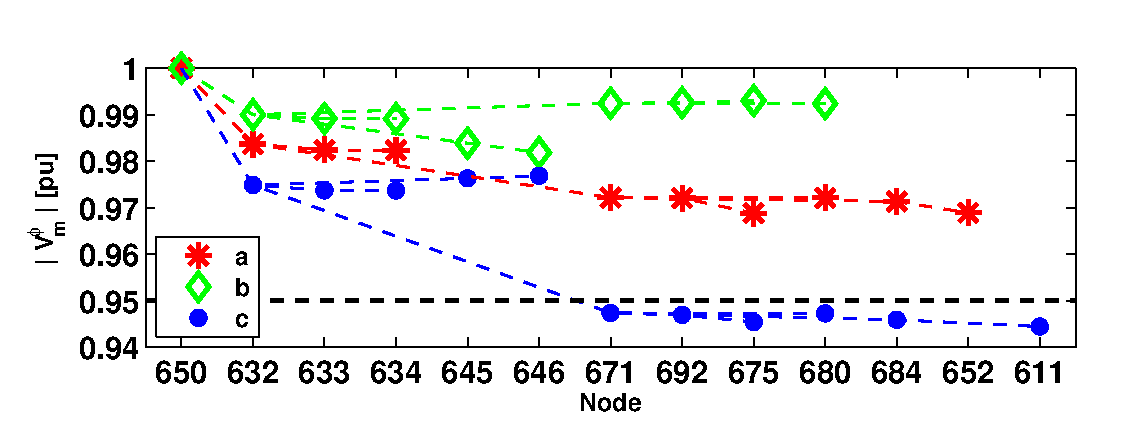
\includegraphics[width=0.49\textwidth]{s2bc}
	\caption{Voltage profile of IEEE 13 node feeder with zero control.}
	\label{fig:s2bc}
    \begin{subfigure}[b]{0.49\textwidth}
        \centering
        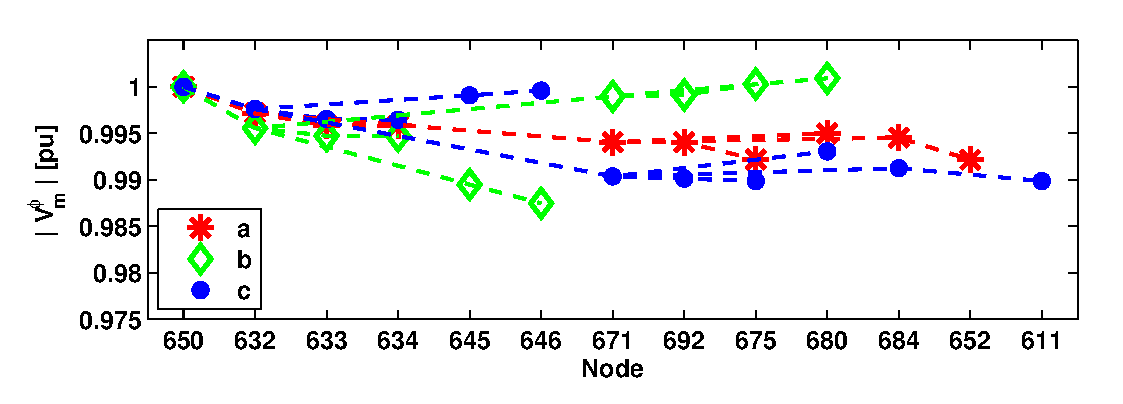
\includegraphics[width=\textwidth]{s1sdp}
        \caption{Voltage profile of IEEE 13 node feeder with SDP control.}
        \label{fig:s1sdp}
    \end{subfigure}
    \\
    \begin{subfigure}[b]{0.49\textwidth}
        \centering
        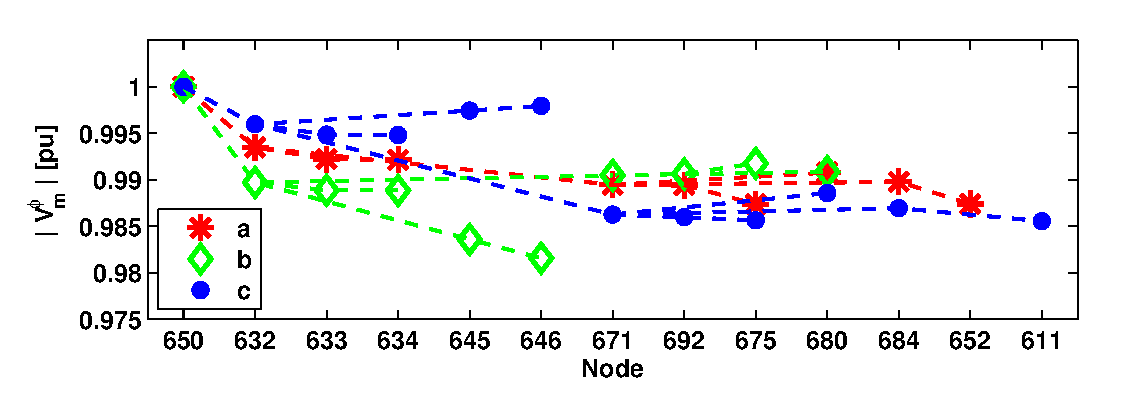
\includegraphics[width=\textwidth]{s1lin}
        \caption{Voltage profile of IEEE 13 node feeder with control from \eqref{eq:OPF1}}
        \label{fig:s1lin}
    \end{subfigure}
    \caption{Comparison of voltage profiles for feeder head real power minimization scenario.}
    \label{fig:s1}
    \begin{subfigure}[b]{0.49\textwidth}
        \centering
        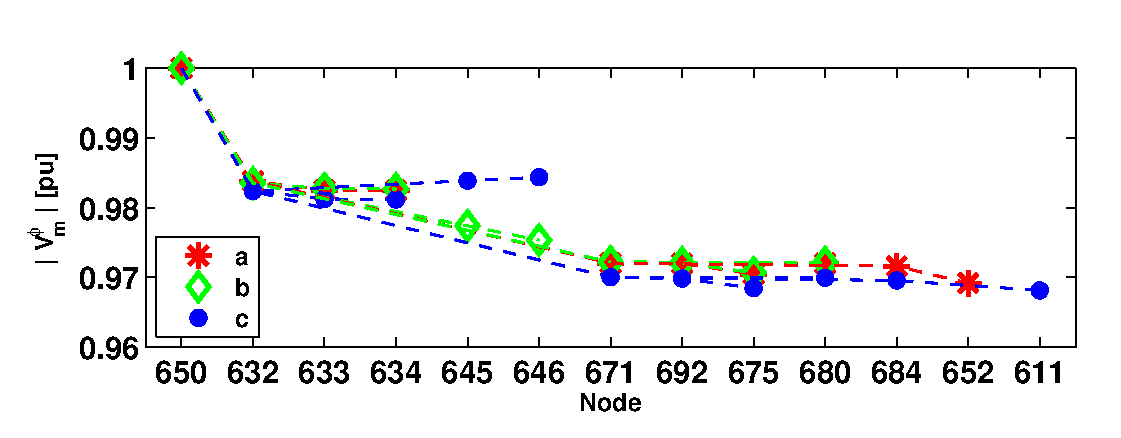
\includegraphics[width=\textwidth]{s2c1}
        \caption{Voltage profile of IEEE 13 node feeder with \eqref{eq:OPF2} Case 1 control.}
        \label{fig:s2c1}
    \end{subfigure}
    \\
    \begin{subfigure}[b]{0.49\textwidth}
        \centering
        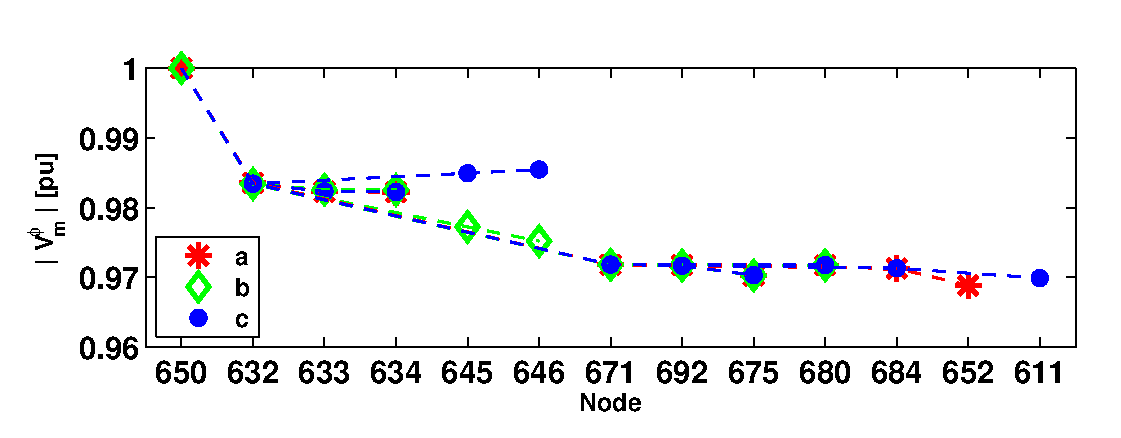
\includegraphics[width=\textwidth]{s2c3}
        \caption{Voltage profile of IEEE 13 node feeder with \eqref{eq:OPF2} Case 2 control.}
        \label{fig:s2c3}
    \end{subfigure}
    \caption{Comparison of voltage profiles for voltage balancing scenario.}
    \label{fig:s2}
\end{figure}

\noindent where $\phi,\psi \in  \{ a,b,c\}$ and $\mathbb{Y}$ is the set of all $\mathbb{Y}_{n}, \text{ } n \in H$. The voltage imbalance for Case 0 is 0.05443. The imbalance for Case 1 is 8.334e-4, and the imbalance for Case 2 is 8.054e-4, a 3.36 \% improvement over Case 1.


% Table \ref{tab:s2} clearly shows the improvement in voltage imbalance over case 0, where no control is applied. It can be seen that case 2 actually performs worse than case 1. This is likely due to the initialization of voltage ratios and loss terms that alter the equality constraints of \eqref{eq:OPF2} from that of case 1. However, the iterative method in case 3 gives the best performance, with voltage imbalance improved 8.28\% over case 1. This can be attributed to updating voltage ratios and $\mathbb{L}_{jk}$, and $\mathbb{H}_{jk}$ at every iteration. Updating these terms alters the the equality constraints of \eqref{eq:OPF2}, in turn providing a current and more realistic set of constraints for the optimal control at the iteration.

% \begin{figure}[t]
% \centering
% \begin{subfigure}[b]{0.49\textwidth}
% 	\centering
% 	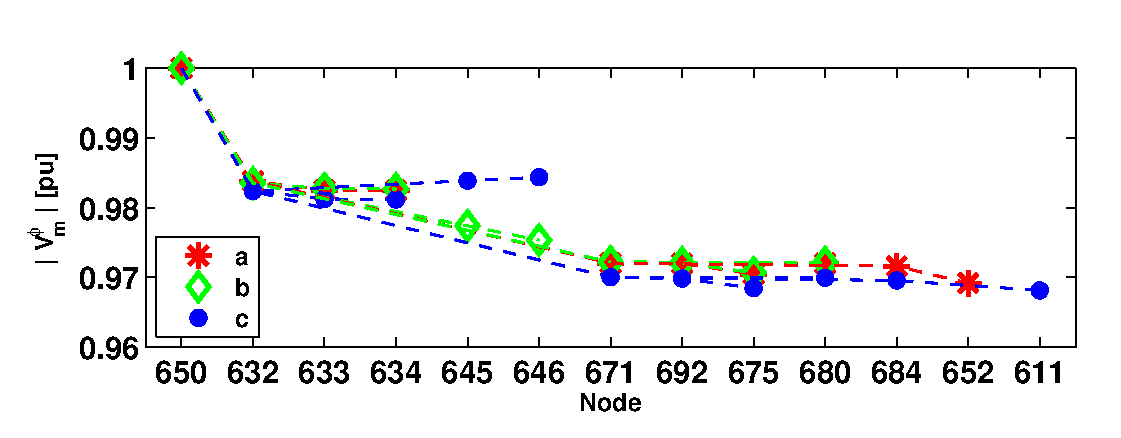
\includegraphics[width=\textwidth]{s2c1}
% 	\caption{Voltage profile of control case 1.}
% 	\label{fig:s2c1}
% \end{subfigure}
% \\
% % \begin{subfigure}[b]{0.49\textwidth}
% % 	\centering
% % 	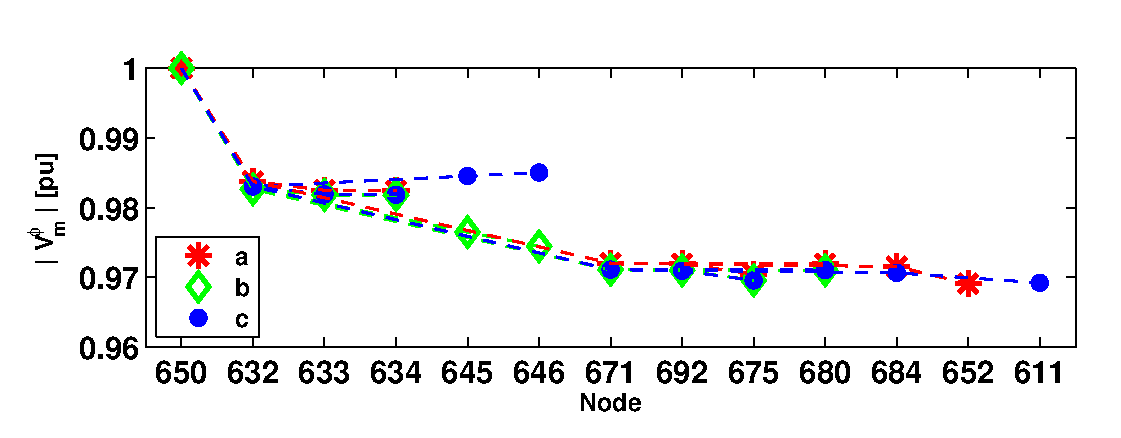
\includegraphics[width=\textwidth]{s2c2}
% % 	\caption{Voltage profile of control case 2.}
% % 	\label{fig:s2c2}
% % \end{subfigure}
% % \\
% \begin{subfigure}[b]{0.49\textwidth}
% 	\centering
% 	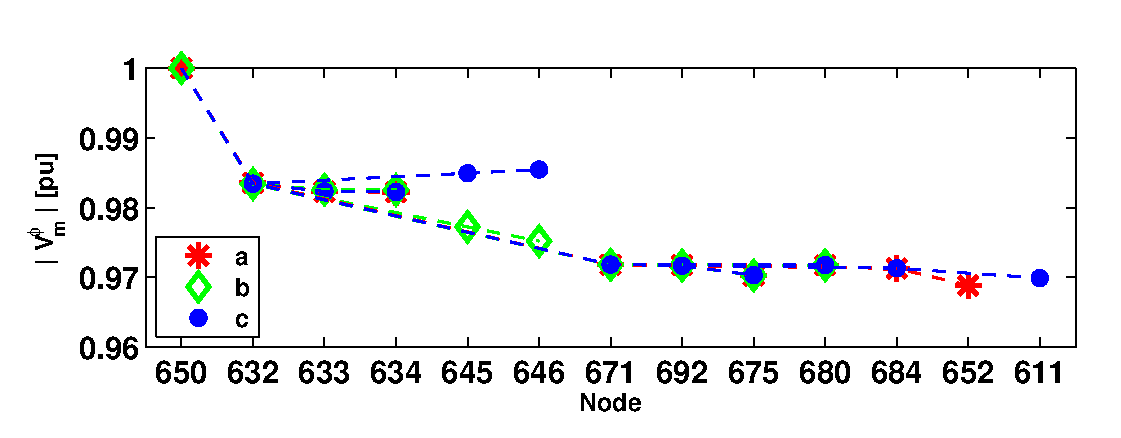
\includegraphics[width=\textwidth]{s2c3}
% 	\caption{Voltage profile of control case 3.}
% 	\label{fig:s2c3}
% \end{subfigure}
% \caption{Voltage profiles for base and three control cases.}
% \label{fig:s2}
% \end{figure}


% \begin{table}[h]
% 	\caption{COMPARISON OF VOLTAGE IMBALANCE}
% 	\begin{center}
% 		\begin{tabular}{| c | c | c |}
%         \hline
%         Case & $J (\mathbb{Y}) \times 1000$ \\
%         \hline
%         0  & 54.43 \\
%         1 & 0.68516 \\
%         2 & 0.6922 \\
%         3 & 0.62847 \\
%         \hline
% \end{tabular}
% \end{center}
% \label{tab:s2}
% \end{table}


